\section{Abstract Factory}

The abstract factory pattern provides a way to encapsulate a group of individual factories that have a common theme without specifying their concrete classes. In normal usage, the client software creates a concrete implementation of the abstract factory and then uses the generic interface of the factory to create the concrete objects that are part of the theme. The client does not know which concrete objects it gets from each of these internal factories since it uses only the generic interfaces of their products. This pattern separates the details of implementation of a set of objects from their general usage and relies on object composition, as object creation is implemented in methods exposed in the factory interface.

\subsection*{Example}

Figure~\ref{fig:abstract_factory} presents the UML diagram of the Abstract Factory design pattern in the project \textit{openjms}. The abstract class \texttt{AbstractHTTPManagedConnectionFactory} plays the role of \textit{abstract factory}, and the class \texttt{HTTPManagedConnectionFactory} plays the role of \textit{concrete factory}. Additionally, \texttt{ConnectionFactory}, \texttt{Managed\\Connection}, and \texttt{ManagedConnectionAcceptor} play the role of \textit{products}.\\

\begin{figure}[htb]
    \centering
    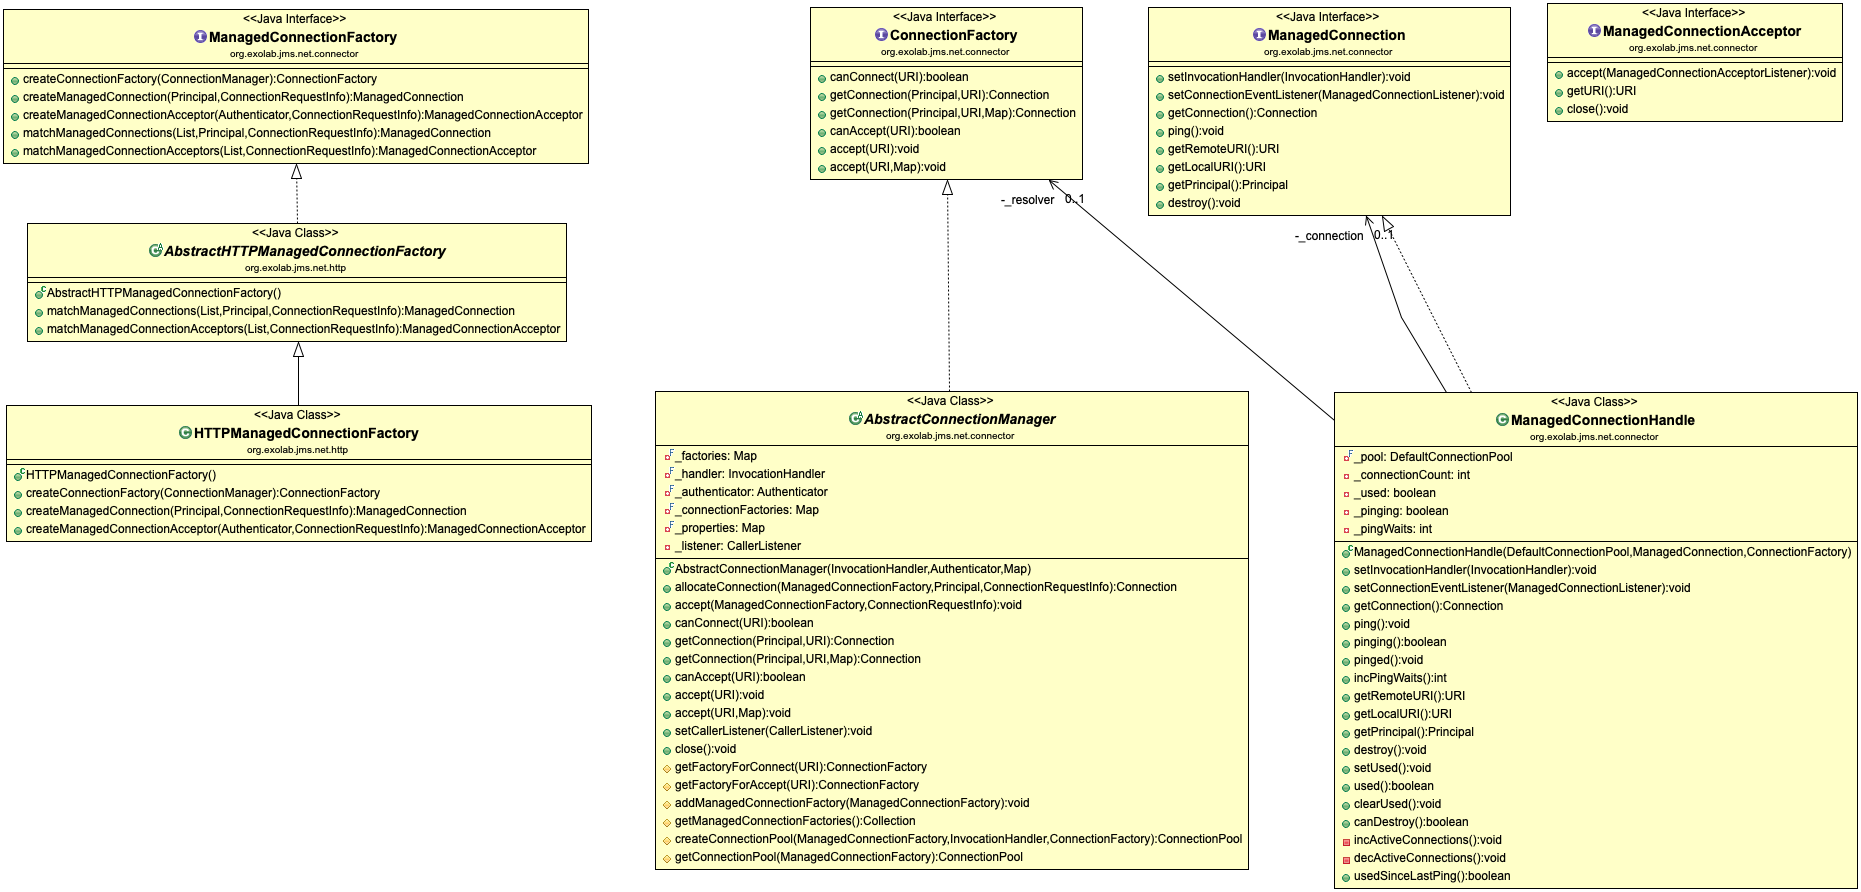
\includegraphics[width=\columnwidth]{images/abstract_factory.png}
    \caption{Abstract Factory design pattern in the project \textit{openjms}}
    \label{fig:abstract_factory}
\end{figure}
\FloatBarrier


An instance of the client class manages the connections. When it determines the connection that needs to be created, it passes the connection request info for the methods \texttt{createConnectionFactory}, \texttt{createManagedConnection}, \texttt{createManagedConnection\\Acceptor} of a \texttt{HTTPManagedConnectionFactory} object. The concrete class \texttt{HTTP\\ManagedConnectionFactory} extends the abstract class \texttt{AbstractHTTPManaged\\ConnectionFactory}. Additionally, the abstract class \texttt{AbstractHTTPManaged\\ConnectionFactory} implements the interface of the factory \texttt{ManagedConnection\\Factory}. The \texttt{Client} object can then use the \texttt{HTTPManagedConnectionFactory} object to create objects that create a new connection factory, a new connection, and an acceptor for connections. Figure~\ref{fig:managedConnectionFactory} presents the interface of the Abstract Factory pattern in the class \texttt{ManagedConnectionFactory}.

%--------------------------------------------------------------------------------------------%

\begin{figure}[htb]
\centering
\lstset{language=Java, basicstyle=\scriptsize, stepnumber=1, showspaces=false, showstringspaces=false,breaklines=true}
\begin{lstlisting}
public interface ManagedConnectionFactory {

    ConnectionFactory createConnectionFactory(ConnectionManager manager) 
        throws ResourceException;

    ManagedConnection createManagedConnection(Principal principal, 
         ConnectionRequestInfo info) throws ResourceException;

    ManagedConnectionAcceptor createManagedConnectionAcceptor(
        Authenticator authenticator, ConnectionRequestInfo info) 
        throws ResourceException;

    ManagedConnection matchManagedConnections(List connections, Principal principal,
        ConnectionRequestInfo info) throws ResourceException;

\end{lstlisting}
\caption{[Abstract Factory] ManagedConnectionFactory.java}
\label{fig:managedConnectionFactory}
\end{figure}
\FloatBarrier

%--------------------------------------------------------------------------------------------%

Figure~\ref{fig:AbstractHTTPManagedConnectionFactory} presents the abstract class that implements the interface \texttt{ManagedConnection\\Factory}.

\begin{figure}[htb]
\centering
\lstset{language=Java, basicstyle=\scriptsize,stepnumber=1, showspaces=false, showstringspaces=false,breaklines=true}
\begin{lstlisting}

public abstract class AbstractHTTPManagedConnectionFactory implements ManagedConnectionFactory {

    public ManagedConnection matchManagedConnections(List connections,
        Principal principal, ConnectionRequestInfo info) throws ResourceException {
        ManagedConnection result = null;

        if (info instanceof HTTPRequestInfo) {
            HTTPRequestInfo requestInfo = (HTTPRequestInfo) info;
            URI uri = URIHelper.convertHostToAddress(requestInfo.getURI());
            Iterator iterator = connections.iterator();
            while (iterator.hasNext()) {
                AbstractHTTPManagedConnection connection =
                        (AbstractHTTPManagedConnection) iterator.next();
                if (connection.hasPrincipal(principal)
                    && (uri.equals(connection.getRemoteURI())
                        || uri.equals(connection.getLocalURI()))) {
                    result = connection;
                    break;
                }
            }
        }
        return result;
    }

    public ManagedConnectionAcceptor matchManagedConnectionAcceptors(
            List acceptors, ConnectionRequestInfo info) throws ResourceException {
        ManagedConnectionAcceptor result = null;

        if (info instanceof SocketRequestInfo) {
            Iterator iterator = acceptors.iterator();
            while (iterator.hasNext()) {
                SocketManagedConnectionAcceptor acceptor =
                        (SocketManagedConnectionAcceptor) iterator.next();
                if (info.equals(acceptor.getRequestInfo())) {
                    result = acceptor;
                    break;
                }
            }
        }
        return result;
    }
}

\end{lstlisting}
\caption{[Abstract Factory] AbstractHTTPManagedConnectionFactory.java}
\label{fig:AbstractHTTPManagedConnectionFactory}
\end{figure}
\FloatBarrier

%--------------------------------------------------------------------------------------------%
Figure~\ref{fig:HTTPManagedConnectionFactory} presents the implementation of \texttt{HTTPManagedConnectionFactory}, the concrete class that extends \texttt{AbstractHTTPManagedConnectionFactory}. In this class, the method \texttt{createConnectionFactory} returns an object of the type \texttt{Connection\\Factory}, the method \texttt{createManagedConnection} returns an object of the type \texttt{HTTPManagedConnection}, and the method \texttt{createManagedConnectionAcceptor} returns an object of the type \texttt{ManagedConnectionAcceptor}. We present below the implementation of such classes. 

\begin{figure}[htb]
\centering
\lstset{language=Java, basicstyle=\scriptsize, stepnumber=1, showspaces=false, showstringspaces=false,breaklines=true}
\begin{lstlisting}


public class HTTPManagedConnectionFactory extends AbstractHTTPManagedConnectionFactory {

    public ConnectionFactory createConnectionFactory(ConnectionManager manager)
            throws ResourceException {
        return new HTTPConnectionFactory(this, manager);
    }

    public ManagedConnection createManagedConnection(Principal principal,
                                                     ConnectionRequestInfo info)
            throws ResourceException {
        if (!(info instanceof HTTPRequestInfo)) {
            throw new ResourceException("Argument 'info' must be of type "
                                        + HTTPRequestInfo.class.getName());
        }

        return new HTTPManagedConnection(principal, (HTTPRequestInfo) info);
    }

    public ManagedConnectionAcceptor createManagedConnectionAcceptor(
            Authenticator authenticator, ConnectionRequestInfo info)
            throws ResourceException {

        if (!(info instanceof SocketRequestInfo)) {
            throw new ResourceException("Argument 'info' must be of type "
                                        + SocketRequestInfo.class.getName());
        }

        return new HTTPManagedConnectionAcceptor(authenticator,
                                                 (SocketRequestInfo) info);
    }

}
\end{lstlisting}
\caption{[Abstract Factory] HTTPManagedConnectionFactory.java}
\label{fig:HTTPManagedConnectionFactory}
\end{figure}
\FloatBarrier

%--------------------------------------------------------------------------------------------%
Figure~\ref{fig:ConnectionFactory} presents the interface of \texttt{ConnectionFactory} and Figure~\ref{fig:AbstractConnectionManager} presents \texttt{Abstract\\ConnectionManager} that implements \texttt{ConnectionFactory}. This class is instantiated in the \texttt{HTTPManagedConnectionFactory} (see Figure~\ref{fig:HTTPManagedConnectionFactory}). It is responsible for managing connection factories, and their corresponding connection pools.

\begin{figure}[htb]
\centering
\lstset{language=Java, basicstyle=\scriptsize, stepnumber=1, showspaces=false, showstringspaces=false,breaklines=true}
\begin{lstlisting}
public interface ConnectionFactory {

    boolean canConnect(URI uri);

    Connection getConnection(Principal principal, URI uri) throws ResourceException;

    Connection getConnection(Principal principal, URI uri, Map properties) throws ResourceException;

    boolean canAccept(URI uri);

    void accept(URI uri) throws ResourceException;

    void accept(URI uri, Map properties) throws ResourceException;

}
\end{lstlisting}
\caption{[Abstract Factory] ConnectionFactory.java}
\label{fig:ConnectionFactory}
\end{figure}
\FloatBarrier

%--------------------------------------------------------------------------------------------%
\begin{figure}[htb]
\centering
\lstset{language=Java, basicstyle=\scriptsize, stepnumber=1, showspaces=false, showstringspaces=false,breaklines=true}
\begin{lstlisting}

public abstract class AbstractConnectionManager implements ConnectionManager, ConnectionFactory {

    // Attributes
       
    public AbstractConnectionManager(InvocationHandler handler, Authenticator authenticator, Map properties) {
        if (handler == null) { throw new IllegalArgumentException("Argument 'handler' is null");}
        if (authenticator == null) {
            throw new IllegalArgumentException(
                    "Argument 'authenticator' is null");
        }
        _handler = handler;
        _authenticator = authenticator;
        _properties = properties;
    }


    public void accept(ManagedConnectionFactory factory, ConnectionRequestInfo info) throws ResourceException {
        ConnectionPool pool = getConnectionPool(factory);
        ManagedConnectionAcceptor acceptor =
                pool.matchManagedConnectionAcceptors(info);
        if (acceptor == null) {
            acceptor = pool.createManagedConnectionAcceptor(_authenticator, info);
            acceptor.accept(pool.getManagedConnectionAcceptorListener());
        }
    }

    public boolean canConnect(URI uri) {
        ConnectionFactory factory = getFactoryForConnect(uri);
        return (factory != null);
    }

    public Connection getConnection(Principal principal, URI uri) throws ResourceException {
        return getConnection(principal, uri, null);
    }

    public Connection getConnection(Principal principal, URI uri, Map properties) throws ResourceException {
        ConnectionFactory factory = getFactoryForConnect(uri);
        if (factory == null) { throw new ResourceException("No connector for URI=" + uri);}
        return factory.getConnection(principal, uri, properties);
    }

    public boolean canAccept(URI uri) {
        ConnectionFactory factory = getFactoryForAccept(uri);
        return (factory != null);
    }

    public void accept(URI uri) throws ResourceException {
        accept(uri, null);
    }

    public void accept(URI uri, Map properties) throws ResourceException {
        ConnectionFactory factory = getFactoryForAccept(uri);
        if (factory == null) {throw new ResourceException("No connector for URI=" + uri);}
        factory.accept(uri, properties);
    }
    
    // Other methods
}

\end{lstlisting}
\caption{[Abstract Factory] AbstractConnectionManager.java}
\label{fig:AbstractConnectionManager}
\end{figure}
\FloatBarrier

%--------------------------------------------------------------------------------------------%
Figure~\ref{fig:ManagedConnection} presents the interface of \texttt{ManagedConnection} and Figure~\ref{fig:ManagedConnectionHandle} presents \texttt{Managed\\ConnectionHandle} that implements \texttt{ManagedConnection}. This class is instantiated in the \texttt{HTTPManagedConnectionFactory} (see Figure~\ref{fig:HTTPManagedConnectionFactory}). It is responsible for handling all connections.

\begin{figure}[htb]
\centering
\lstset{language=Java, basicstyle=\scriptsize, stepnumber=1, showspaces=false, showstringspaces=false,breaklines=true}
\begin{lstlisting}

public interface ManagedConnection {

    void setInvocationHandler(InvocationHandler handler) throws ResourceException;

    void setConnectionEventListener(ManagedConnectionListener listener) throws ResourceException;

    Connection getConnection() throws ResourceException;

    void ping() throws ResourceException;

    URI getRemoteURI() throws ResourceException;

    URI getLocalURI() throws ResourceException;

    Principal getPrincipal() throws ResourceException;

    void destroy() throws ResourceException;

}
\end{lstlisting}
\caption{[Abstract Factory] ManagedConnection.java}
\label{fig:ManagedConnection}
\end{figure}
\FloatBarrier

%--------------------------------------------------------------------------------------------%

\begin{figure}[htb]
\centering
\lstset{language=Java, basicstyle=\scriptsize, stepnumber=1, showspaces=false, showstringspaces=false,breaklines=true}
\begin{lstlisting}

final class ManagedConnectionHandle implements ManagedConnection {

    public void setInvocationHandler(InvocationHandler handler)
            throws ResourceException {
        _connection.setInvocationHandler(handler);
    }

     public void setConnectionEventListener(ManagedConnectionListener listener)
            throws ResourceException {
        _connection.setConnectionEventListener(listener);
    }

    public Connection getConnection() throws ResourceException {
        Connection connection = _connection.getConnection();
        return new ConnectionHandle(connection);
    }
    
    public synchronized void ping() throws ResourceException {
        try {
            _pinging = true;
            _pingWaits = 0;
            _connection.ping();
        } catch (ResourceException exception) {
            _pinging = false;
            throw exception;
        }
    }
    
    public URI getRemoteURI() throws ResourceException {
        return _connection.getRemoteURI();
    }
    
    public URI getLocalURI() throws ResourceException {
        return _connection.getLocalURI();
    }
    
    public Principal getPrincipal() throws ResourceException {
        return _connection.getPrincipal();
    }
    
    public void destroy() throws ResourceException {
        _connection.destroy();
    }
    
    // Other methods

}

\end{lstlisting}
\caption{[Abstract Factory] ManagedConnectionHandle.java}
\label{fig:ManagedConnectionHandle}
\end{figure}
\FloatBarrier

%--------------------------------------------------------------------------------------------%

Figure~\ref{fig:ManagedConnectionAcceptor} presents the interface of \texttt{ManagedConnectionAcceptor}. 
Although \texttt{Managed\\ConnectionAcceptor} is instantiated in \texttt{HTTPManagedConnectionFactory} (see Figure~\ref{fig:HTTPManagedConnectionFactory}), we could not find any class that implements this interface.

\begin{figure}[htb]
\centering
\lstset{language=Java, basicstyle=\scriptsize, stepnumber=1, showspaces=false, showstringspaces=false,breaklines=true}
\begin{lstlisting}

public interface ManagedConnectionAcceptor {

    void accept(ManagedConnectionAcceptorListener listener)
            throws ResourceException;

    URI getURI() throws ResourceException;
    
    void close() throws ResourceException;
}
\end{lstlisting}
\caption{[Abstract Factory] ManagedConnectionAcceptor.java}
\label{fig:ManagedConnectionAcceptor}
\end{figure}
\FloatBarrier